
%----------------------------------------------------------------------------------------
%	PREAMBUŁA
%----------------------------------------------------------------------------------------

\documentclass[12pt]{article}
\usepackage[polish]{babel}
\usepackage{polski}
\usepackage[utf8]{inputenc}
\usepackage{graphicx}
\usepackage{fancyhdr}
\usepackage{float}
\usepackage{graphicx}
\usepackage[hidelinks]{hyperref}
\usepackage{verbatim}
\usepackage{amsmath}
\usepackage{rotating}
\usepackage{listings}
\usepackage{xcolor}

\definecolor{lgray}{gray}{0.96}
\definecolor{lbcolor}{rgb}{0.9,0.9,0.9}
\lstset{
    framesep=2pt,
    breaklines=true,
    breakatwhitespace=true,
    basicstyle=\footnotesize,
    aboveskip={0.75\baselineskip},
    columns=fixed,
    showstringspaces=false,
    breaklines=true,
    prebreak = \raisebox{0ex}[0ex][0ex]{\ensuremath{\hookleftarrow}},
    frame=single,
    rulecolor=\color{lgray},
    showtabs=false,
    showspaces=false,
    showstringspaces=false,
    backgroundcolor=\color{lgray},
    identifierstyle=\ttfamily,
    keywordstyle=\color[rgb]{0,0,1},
    commentstyle=\color[rgb]{0.0,0.26,0.15},
    stringstyle=\color[rgb]{0.627,0.126,0.941}
}

\graphicspath{{static/}} 

\title{Algorytm Dijkstry}
\author{Arkadiusz Kasprzak, Aleksandra Poręba}

\makeatletter
\let\thetitle\@title
\let\theauthor\@author
\let\thedate\@date
\makeatother

%----------------------------------------------------------------------------------------
%	STRONA TYTUŁOWA
%----------------------------------------------------------------------------------------
\begin{document}
\begin{center}
\textsc{\normalsize Wydział Fizyki i Informatyki Stosowanej}\\[2.0cm] 

\includegraphics[scale = 1]{logo.pdf}\\[1cm] 
\textsc{\Large Systemy równoległe i rozproszone}\\[0.4cm] 


{ \huge \bfseries \LARGE{Drzewa wszystkich najkrótszych ścieżek - algorytm Dijkstry} }\\[0.2cm] 
{ \huge \bfseries \LARGE{Aplikacja równoległa MPI} }\\[1cm] 

\flushright \Large Arkadiusz Kasprzak \\ Aleksandra Poręba

\vfill 

\center {\today}\\[2cm] 


\pagebreak 

\end{center}

%----------------------------------------------------------------------------------------
%	SPIS TREŚCI
%----------------------------------------------------------------------------------------
\setcounter{tocdepth}{2}
\tableofcontents
\pagebreak

%----------------------------------------------------------------------------------------
%	ZAWARTOŚĆ
%----------------------------------------------------------------------------------------

\pagestyle{fancy}
\fancyhf{}

\rhead{\theauthor}
\lhead{\thetitle}
\cfoot{\thepage}

\section{Wstęp}
Niniejszy dokument stanowi dokumentację projektu wykonanego w ramach przedmiotu \textit{Systemy równoległe i rozproszone}. Tematem projektu było stworzenie, z użyciem protokołu MPI, aplikacji równoległej implementującej algorytm Dijkstry.

\subsection{Algorytm Dijkstry}
Zaimplementowany w ramach projektu algorytm Dijkstry jest algorytmem poszukiwania najkrótszych ścieżek z wybranego wierzchołka do wszystkich pozostałych w grafie (skierowanym lub nieskierowanym) o nieujemnych wagach krawędzi. Oparty jest on na metodzie zachłannej: w każdym kroku wybierany jest wierzchołek, do którego koszt dojścia jest najmniejszy. 

\begin{lstlisting}[caption={Pseudokod algorytmu Dijkstry.}, captionpos=b, mathescape=true, basicstyle=\scriptsize]
V - zbior wierzcholkow
E - zbior krawedzi z wagami
v - wierzcholek startowy

Dijkstra(V, E, v)
    Q := $\emptyset$;
    p := -1;
    d := $\infty$
    d(v) := 0
    dopoki Q != V wykonaj
        wybierz spoza zbioru Q wierzcholek u o najmniejszym koszcie d(u)
        Q := Q $\cup$ {u}
        dla kazdego sasiada w wierzcholka u spoza zbioru Q wykonaj
            jesli d(w) > d(u) + E(w, u) to
                d (w) :=  d(u) + E(w, u)
                p(w) := u
\end{lstlisting}

W czasie wykonania algorytmu program operuje na dwóch tablicach - jedna z nich, zwykle oznaczana literą \lstinline{d}, przechowuje koszty dotarcia z wierzchołka źródłowego do każdego z wierzchołków w badanym grafie. Druga, oznaczana literą \lstinline{p}, przechowuje informację o poprzedniku każdego z wierzchołków - taka informacja pozwala po zakończeniu działania algorytmu odtworzyć ścieżkę z wierzchołka źródłowego do każdego z wierzchołków w grafie.

\subsection{Aplikacje równoległe MPI}
Aplikacje równoległe charakteryzują się możliwością działania na wielu procesorach (rdzeniach) równocześnie. Wiąże się to z podziałem problemu na mniejsze fragmenty, które mogą wykonywać się niezależnie od siebie. Wynik działania programu powstaje przez połączenie poszczególnych rozwiązań.

Do implementacji aplikacji rozproszonych powstał standard MPI (\textit{Message Passage Interface}), który stanowi protokół komunikacyjny pomiędzy równoległymi procesami. Odbywa się to za pomocą jawnie przekazywanych komunikatów. Możliwe są różne rodzaje komunikacji, na przykład typu punkt-punkt pomiędzy dwoma procesami (\lstinline|MPI_Send|, \lstinline|MPI_Recv|), albo komunikacja grupowa, gdzie bierze udział wiele procesów (na przykład \lstinline|MPI_Bcast|, \lstinline|MPI_Reduce|). Standard MPI jest wysocy wydajny i umożliwia efektywną obsługą dużej ilości procesów.

W projekcie została użyta biblioteka \lstinline|MPICH| będąca implementacją standardu MPI.

\newpage
\section{Budowa projektu}
W tej części dokumentacji opisana została budowa przygotowanego projektu - zarówno jeśli chodzi o podział projektu na komponenty (biblioteki), jak i na poszczególne klasy. Nie jest to natomiast dokumentacja kodu - ta została przygotowana odrębnie, w postaci zbioru dokumentów HTML, przy pomocy narzędzia \lstinline{Doxygen}.

\subsection{Podział na komponenty}
Projekt podzielony został na trzy główne komponenty:
\begin{itemize}
\item \lstinline{DijkstraCommon} - biblioteka statyczna zawierająca klasy oraz funkcje współdzielone przez pozostałe dwa komponenty. W jej skład wchodzą klasy odpowiedzialne za: zapis wyników obliczeń, walidację danych podanych przez użytkownika, przechowywanie danych na temat przetwarzanego grafu i jego poszczególnych wierzchołków czy przetwarzanie argumentów linii poleceń. Zawiera również klasę \lstinline{DijkstraAlgorithmBackend} stanowiącą szkielet implementowanego algorytmu.
\item \lstinline{DijkstraSerial} - implementacja algorytmu bez użycia protokołu MPI, czyli w formie klasycznego algorytmu szeregowego. Komponent ten został dołączony do projektu jako punkt odniesienia w procesie testowania wydajności implementacji równoległej. Zawiera funkcję \lstinline{main}.
\item \lstinline{DijkstraMPI} - implementacja algorytmu używająca protokołu MPI. Jest to jedyny komponent projektu używający tej biblioteki. Zawiera funkcję \lstinline{main}.
\end{itemize}
\begin{figure}[H]
\centering
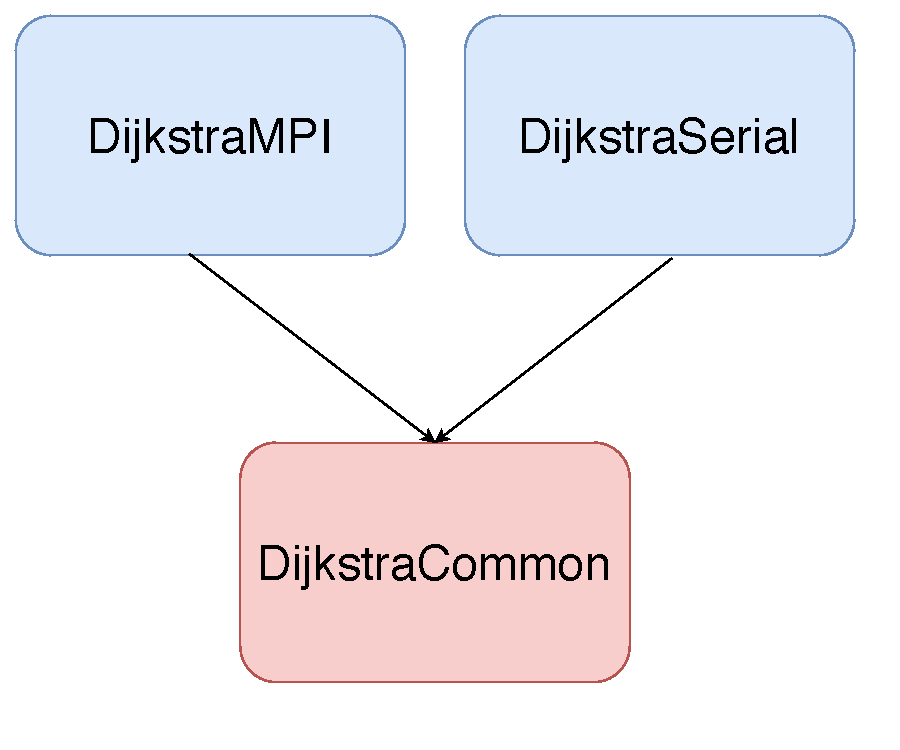
\includegraphics[width=0.35\textwidth]{static/DijkstraArch1.pdf}
\caption{Komponenty wchodzące w skład projektu wraz z wzajemnymi zależnościami.}
\label{fig:arch1}
\end{figure}

Zależności między poszczególnymi komponentami przedstawia rysunek \ref{fig:arch1}. Na niebiesko oznaczone zostały komponenty produkujące plik wykonywalny, na czerwono natomiast biblioteki. Każdy z komponentów znajduje się w osobnym katalogu o nazwie odpowiadającej nazwie komponentu.


\subsection{Najważniejsze klasy w projekcie}
Poniżej przedstawiono listę najważniejszych klas wchodzących w skład projektu (nie jest to pełna lista wszystkich klas, taką listę znaleźć można w dokumentacji wygenerowanej za pomocą narzędzia \lstinline{Doxygen}):
\begin{itemize}
\item klasa \lstinline{DijkstraAlgorithmBackend} z komponentu \lstinline{DijkstraCommon} - stanowi podstawę implementacji algorytmu zarówno w przypadku równoległym, jak i sekwencyjnym. Zarządza stanem wykonania algorytmu i wykonuje na tym stanie podstawowe operacje przewidziane przez algorytm, np. dodanie wierzchołka do zbioru wierzchołków przetworzonych czy wybór wierzchołka o najniższym koszcie. 
\item klasa \lstinline{DijkstraMPI} z komponentu \lstinline{DijkstraMPI} - zawiera równoległą implementację algorytmu Dijkstry. Korzysta z API udostępnionego przez klasę \lstinline{DijkstraAlgorithmBackend}. Dostarcza pojedynczą metodę \lstinline{run} wykonującą algorytm i zwracającą jego wynik.
\item klasa \lstinline{DijkstraSerial} z komponentu \lstinline{DijkstraSerial} - zawiera sekwencyjną implementację algorytmu Dijkstry. Korzysta z API udostępnionego przez klasę \lstinline{DijkstraAlgorithmBackend}. Dostarcza pojedynczą metodę \lstinline{run} wykonującą algorytm i zwracającą jego wynik.
\item klasa \lstinline{AdjacencyMatrix} z komponentu \lstinline{DijkstraCommon} - pozwala na wczytanie i przechowywanie danych wejściowych
\item klasa szablonowa \lstinline{Log} - udostępnia opcję wypisywania na standardowe wyjście informacji na temat działania algorytmu. Posiada specjalizację \lstinline{Log<false>}, które wyłącza mechanizm wypisywania informacji. Implementacja wypisywania oparta jest na tzw. \textit{variadic templates} z C++11. 
\end{itemize}

\newpage
\section{Działanie projektu}
W tej części dokumentacji omówiony zostanie sposób działania implementacji algorytmu Dijkstry wykorzystującej protokół MPI. Algorytm składa się z trzech głównych części:
\begin{itemize}
\item inicjalizacja - podział danych wejściowych na części, walidacja, rozesłanie danych do poszczególnych procesów
\item obliczenie odległości i ścieżek (algorytm Dijkstry)
\item zapisanie wyników do pliku i zakończenie działania programu
\end{itemize}


\subsection{Inicjalizacja}
Pierwsza część programu składa się z kilku mniejszych etapów. Na początku ma miejsce standardowa inicjalizacja protokołu MPI oraz przypisanie każdemu z procesów rangi. Kolejnym etapem jest utworzenie klasy odpowiedzialnej za wyświetlanie informacji o przebiegu programu na standardowe wyjście. W dalszej kolejności przetwarzane i walidowane są dane wejściowe - numer wierzchołka stanowiącego źródło oraz ścieżka do pliku z danymi wejściowymi. W przypadku, gdy dane są niepoprawne, program kończy działanie wyświetlając odpowiedni komunikat.

\vspace{5mm}
Następnie odbywa się przede wszystkim podział danych wejściowych na części i rozesłanie ich do poszczególnych procesów. Program przyjmuje informacje na temat przetwarzanego grafu w postaci tzw. \textbf{macierzy sąsiedztwa}. W i-tym rzędzie i j-tej kolumnie takiej macierzy znajduje się waga przypisana do krawędzi łączącej wierzchołek $i$ z wierzchołkiem $j$. W przypadku braku krawędzi waga wynosi 0. Rysunek \ref{fig:am1} przedstawia przykład tego typu reprezentacji wraz z odpowiadającym jej grafem.

\begin{figure}[H]
\centering
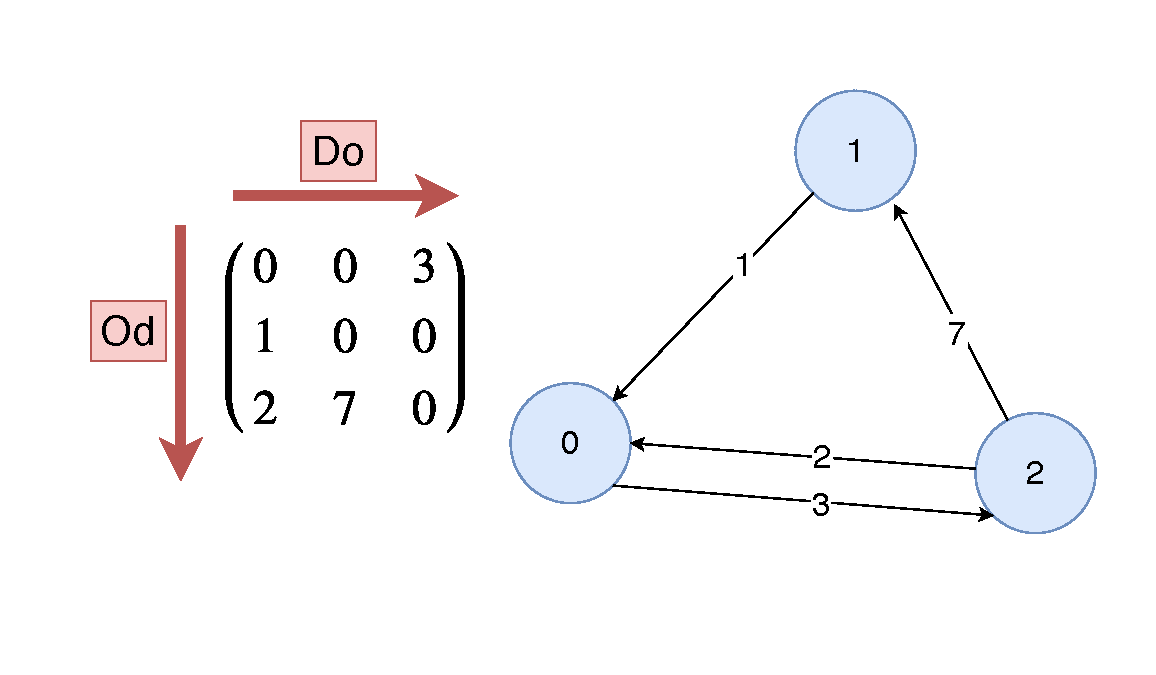
\includegraphics[width=\textwidth]{static/AdjacencyMatrixExample.pdf}
\caption{Przykładowa macierz sąsiedztwa wraz z odpowiadającym jej grafem skierowanym.}
\label{fig:am1}
\end{figure}

Macierz sąsiedztwa wczytywana jest z pliku z danymi wejściowymi przez proces główny (proces \lstinline{root} o identyfikatorze 0). Proces ten dokonuje podziału macierzy na części zgodnie z ilością procesów biorących udział w wykonaniu algorytmu. Każdy z procesów otrzymuje k kolumn oryginalnej macierzy w formie ciągłego obszaru pamięci - przykładowy podział dla grafu o 5 wierzchołkach i 3 procesów przedstawia rysunek \ref{fig:am2}.

\vspace{5mm}
Algorytm podziału jest prosty. Dana jest macierz o $n$ kolumnach i $m$ procesów. Najpierw każdemu z procesów przypisywane jest:
\begin{equation}
a = \left\lfloor \frac{n}{m} \right\rfloor
\end{equation}
kolumn - w przypadku $n = 5$ i $m = 3$ każdy proces otrzymuje domyślnie jedną kolumnę. Ilość pozostałych kolumn dana jest zależnością:
\begin{equation}
k = n \mod m
\end{equation}
W analizowanym przykładzie jest to $k = 2$. Kolumny te rozdzielane są po jednej pomiędzy k pierwszych (zgodnie z numeracją nadaną przez MPI) procesów. Ostatecznie w omawianym przykładzie proces zerowy i pierwszy otrzymują po dwie kolumny, proces drugi otrzymuje natomiast tylko jedną kolumnę.

\begin{figure}[H]
\centering
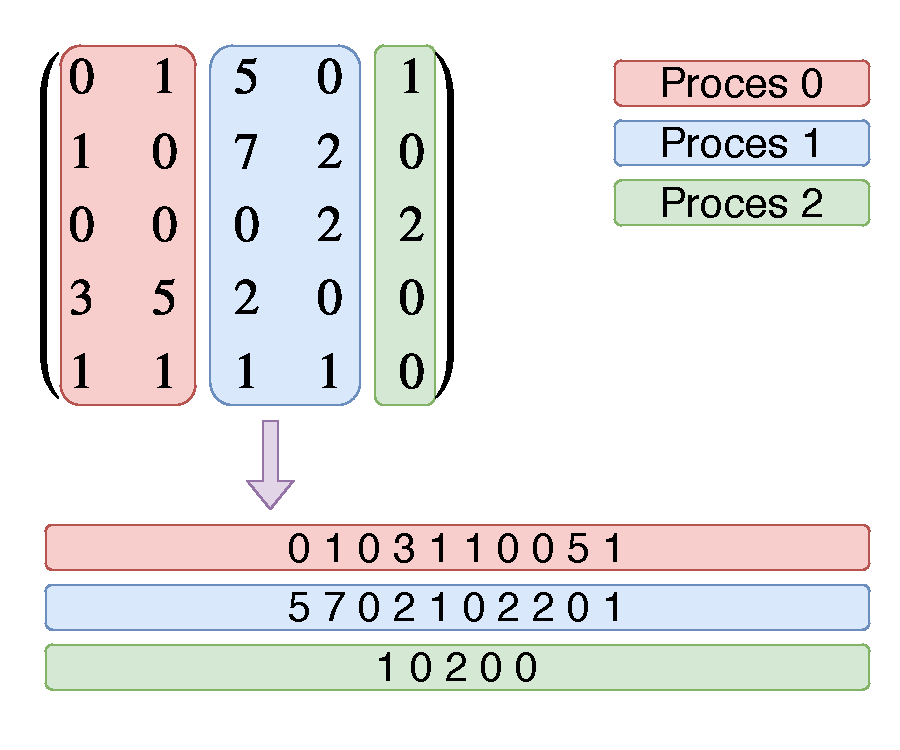
\includegraphics[width=\textwidth]{static/MatrixSplit.pdf}
\caption{Przykładowy podział macierzy sąsiedztwa reprezentującej graf o 5 wierzchołkach. W wykonaniu algorytmu biorą udział 3 procesy.}
\label{fig:am2}
\end{figure}

Kolumny przypisywane są każdemu procesowi po kolei, tzn. proces 0 otrzymuje $x_0$ pierwszych kolumn macierzy, proces 1 kolejne $x_1$ itd. Zbiór kolumn reprezentowany jest za pomocą jednowymiarowej tablicy - ułożone są w niej kolejno dane z pierwszej, drugiej itd. kolumny.

\newpage
Po dokonaniu przez proces \lstinline{root} podziału, do każdego z procesów wysyłane są trzy informacje:
\begin{itemize}
\item całkowita liczba wierzchołków w przetwarzanym grafie - wysyłanie odbywa się za pomocą operacji kolektywnej \lstinline{MPI_Bcast}
\item ilość kolumn macierzy sąsiedztwa, jaka każdy z procesów będzie musiał obsłużyć. Informacja ta jest w tym momencie potrzebna, ponieważ każdy z procesów musi przygotować sobie odpowiednio duży bufor na dane z samej macierzy. Wysyłanie tej informacji odbywa się za pomocą operacji \lstinline{MPI_Scatter}, ponieważ każdy z procesów otrzymuje swoją indywidualną informację.
\item zawartość kolumn macierzy sąsiedztwa, które będą przetwarzane przez dany proces. Wysyłanie tej informacji odbywa się za pomocą funkcji \lstinline{MPI_Scatterv}, ponieważ jest ona w stanie obsłużyć wysyłanie innej ilości danych do każdego z procesów.
\end{itemize}

Po zakończeniu wysyłania danych następuje podział procesów na dwie grupy: procesy które otrzymały przynajmniej jedną kolumnę oraz takie, które nie otrzymały żadnej (ma to miejsce, gdy do wykonania algorytmu przydzielone zostaje więcej procesów, niż przetwarzany graf posiada wierzchołków). W tym celu za pomocą operacji \lstinline{MPI_Comm_split} komunikator globalny dzielony jest na dwa komunikatory. Kryterium podziału stanowi tutaj właśnie sprawdzenie, czy procesowi zostały przydzielone kolumny macierzy do obsługi (\lstinline{numberOfColumnsToHandle > 0}). Pozwala to wykluczyć nadmiarowe procesy z dalszego przebiegu algorytmu.

\vspace{5mm}
Przebieg procesu inicjalizacji jest komunikowany użytkownikowi - na standardowym wyjściu pojawiają się odpowiednie informacje. Poniżej zamieszczono przykład takich informacji wygenerowany dla przykładu widocznego na rysunku \ref{fig:am2}:

\begin{lstlisting}
[Process 0] This process will handle 2 vertices in range [0, 1]
[Process 1] This process will handle 2 vertices in range [2, 3]
[Process 2] This process will handle 1 vertices in range [4, 4]
...
\end{lstlisting}

Rysunek \ref{fig:diagram1} przedstawia \textbf{schemat blokowy} ilustrujący przebieg procesu inicjalizacji.

\begin{figure}[H]
\centering
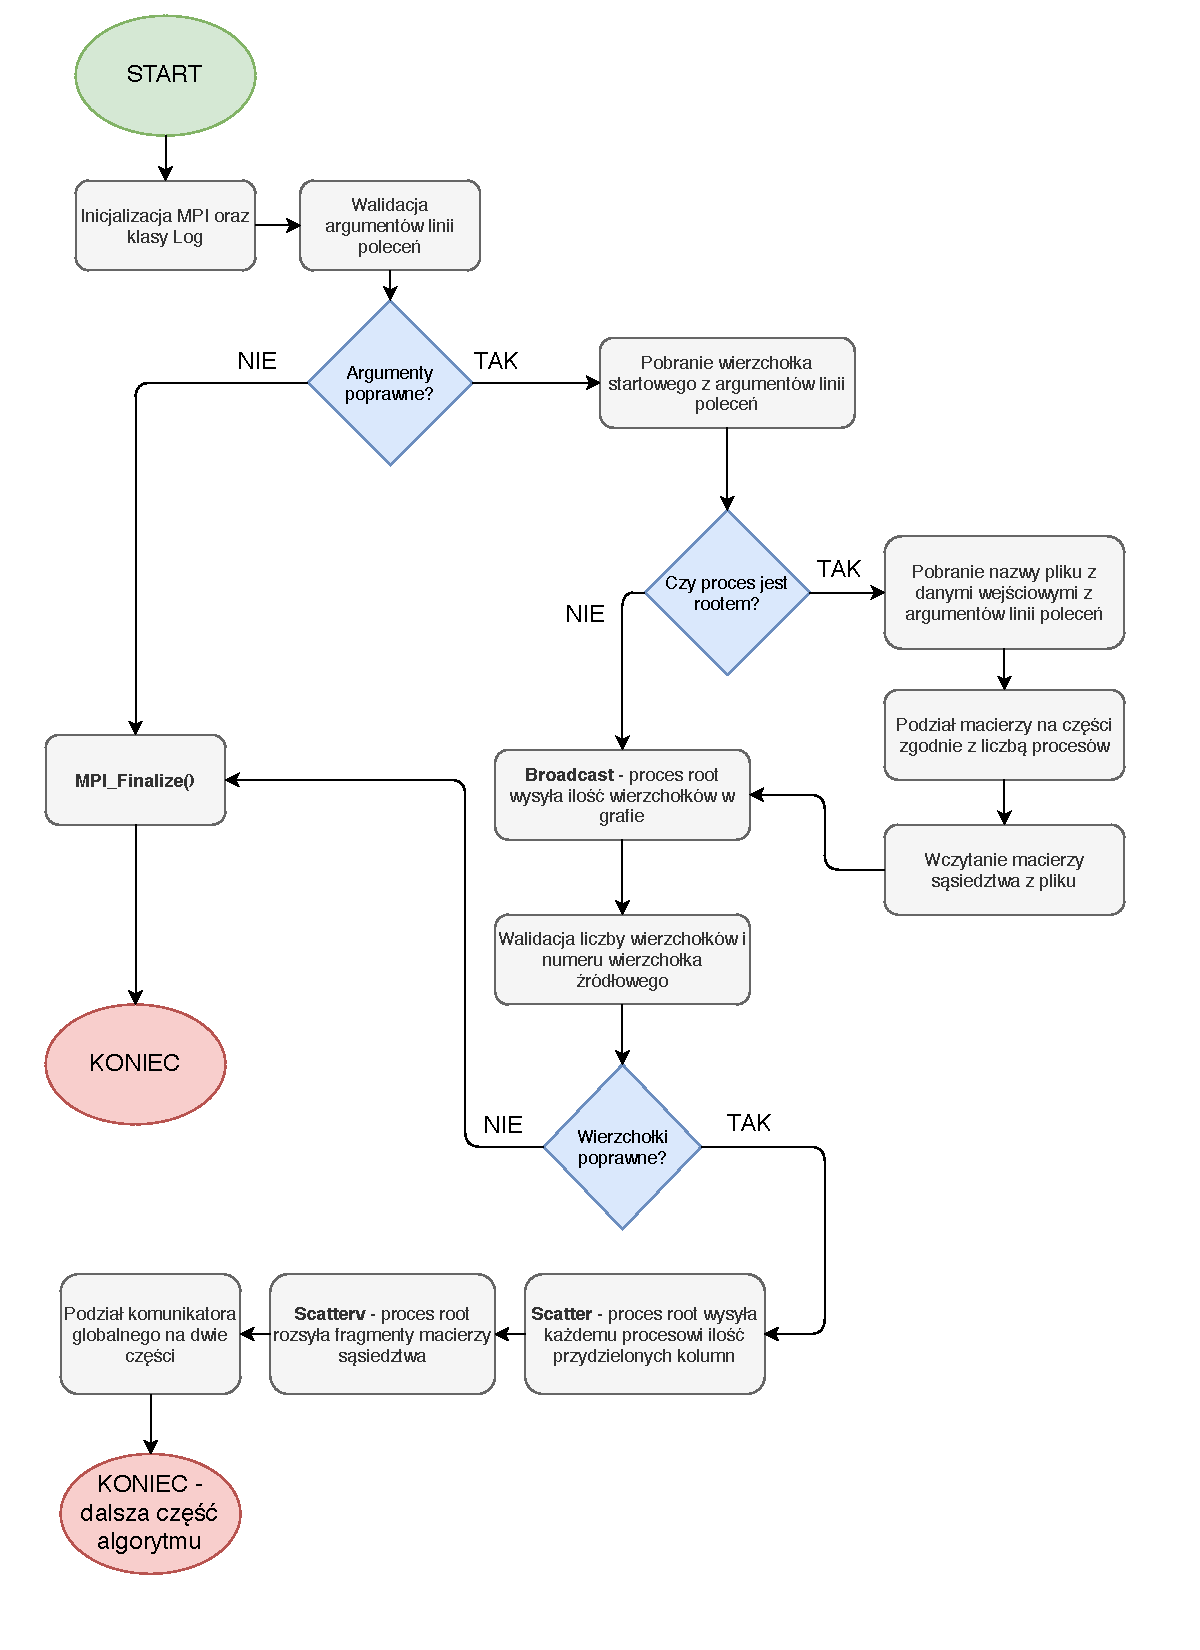
\includegraphics[width=\textwidth]{static/Diagram1.pdf}
\caption{Schemat blokowy ilustrujący przebieg procesu inicjalizacji.}
\label{fig:diagram1}
\end{figure}


\subsection{Implementacja i zakończenie algorytmu}
Początek właściwej części programu stanowi sprawdzenie, czy danemu procesowi przydzielone zostały wierzchołki grafu (czyli kolumny macierzy sąsiedztwa) do przetworzenia. Jeśli nie, to taki proces nie bierze udziału w dalszym wykonaniu algorytmu - następuje dealokacja utworzonego komunikatora i zakończenie działania. W przeciwnym wypadku proces przystępuje do realizacji algorytmu. 

\vspace{5mm}
Implementacja algorytmu Dijkstry za pomocą protokołu MPI nie różni się w sposób znaczący od klasycznej implementacji szeregowej. Każdy z procesów obsługuje dwie tablice: 
\begin{itemize}
\item tablica odległości (kosztów) od wierzchołka źródłowego do każdego z wierzchołków w grafie
\item tablica poprzedników każdego z wierzchołków - służy do odtworzenia najkrótszych ścieżek między wierzchołkami
\end{itemize}
oraz zbiór obsłużonych wierzchołków (często nazywany klastrem). Początkowo zbiór ten jest pusty, tablica kosztów zainicjalizowana jest nieskończonościami, a tablica poprzedników wartościami -1. Różnica w stosunku to szeregowej wersji algorytmu jest taka, że w przypadku implementacji równoległej każdy z procesów przechowuje \textbf{fragmenty tych tablic} odpowiadające przydzielonym im wierzchołkom grafu.

\vspace{5mm}
W procesie obsługującym wierzchołek źródłowy jego wpis w tablicy kosztów ustawiany jest na wartość 0. Następnie, dopóki wszystkie wierzchołki nie zostały przetworzone, wykonywany jest w pętli algorytm:
\begin{itemize}
\item każdy proces wybiera spośród przydzielonych mu wierzchołków taki, który nie został jeszcze dodany do zbioru wierzchołków obsłużonych i którego wartość w tablicy kosztów jest najmniejsza
\item za pomocą operacji \lstinline{MPI_Allreduce} wybierany jest wierzchołek o globalnie najniższej wartości kosztu (czyli najlepszy spośród najlepszych z każdego procesu)
\item jeśli nie został wyznaczony taki wierzchołek, to następuje wyjście z pętli i zakończenie algorytmu
\item w przeciwnym razie wierzchołek zostaje dodany do zbioru wierzchołków przetworzonych (w każdym procesie zbiór ten jest przechowywany osobno, w całości)
\item dla każdego nieprzetworzonego sąsiada wyznaczonego wierzchołka dokonywana jest aktualizacja w tablicy kosztów i poprzedników (wybrany wierzchołek staje się poprzednikiem swoich sąsiadów), jeśli nowy koszt okazuje się niższy od dotychczasowego
\end{itemize}
Po zakończeniu działania algorytmu fragmenty tablic kosztów i poprzedników są łączone w całość za pomocą operacji \lstinline{MPI_Gatherv}. Proces \lstinline{root} wyznacza ścieżki z wierzchołka źródłowego do każdego wierzchołka w grafie i zapisuje wyniki do pliku. Następnie wyświetlany jest czas działania algorytmu. Ostatnim krokiem jest zwolnienie utworzonego wcześniej komunikatora, wywołanie operacji \lstinline{MPI_Finalize} i zakończenie działania programu.

\vspace{5mm}
W kilku miejscach w programie tworzona jest zmienna zawierająca aktualny czas. Pod koniec działania, proces \lstinline{root} zbiera te informacje i wyświetla czas wykonywania się każdej z trzech części programu:
\begin{lstlisting}
[Process 0] Total elapsed time: 0.0298846s
[Process 0] Setup took: 0.0260188s
[Process 0] Algorithm took: 0.0020106s
[Process 0] Printing solution took: 0.0018552s
\end{lstlisting}
Wyświetlane są wyniki pomiarów dokonanych jedynie w procesie głównym - wyniki z pozostałych procesów są pomijane. Pomiar wykonywany jest z użyciem obiektu klasy \lstinline{high_resolution_clock} z biblioteki \lstinline{chrono} (standard C++11). Użycie takiego zegara gwarantuje, że mierzony czas jest czasem rzeczywistym, a nie czasem procesora.

\vspace{5mm}
Rysunek \ref{fig:diagram2} przedstawia schemat blokowy ilustrujący przebieg działania algorytmu po inicjalizacji. Kolorem fioletowym oznaczony został blok związany z główną pętlą algorytmu Dijkstry. Schemat ten nie zawiera szczegółów jej działania.

\vspace{5mm}
Rysunek \ref{fig:diagram3} przedstawia schemat blokowy ilustrujący działania głównej pętli algorytmu Dijkstry. Schemat ten stanowi rozwinięcie fioletowego bloku z rysunku \ref{fig:diagram2}.

\begin{figure}[H]
\centering
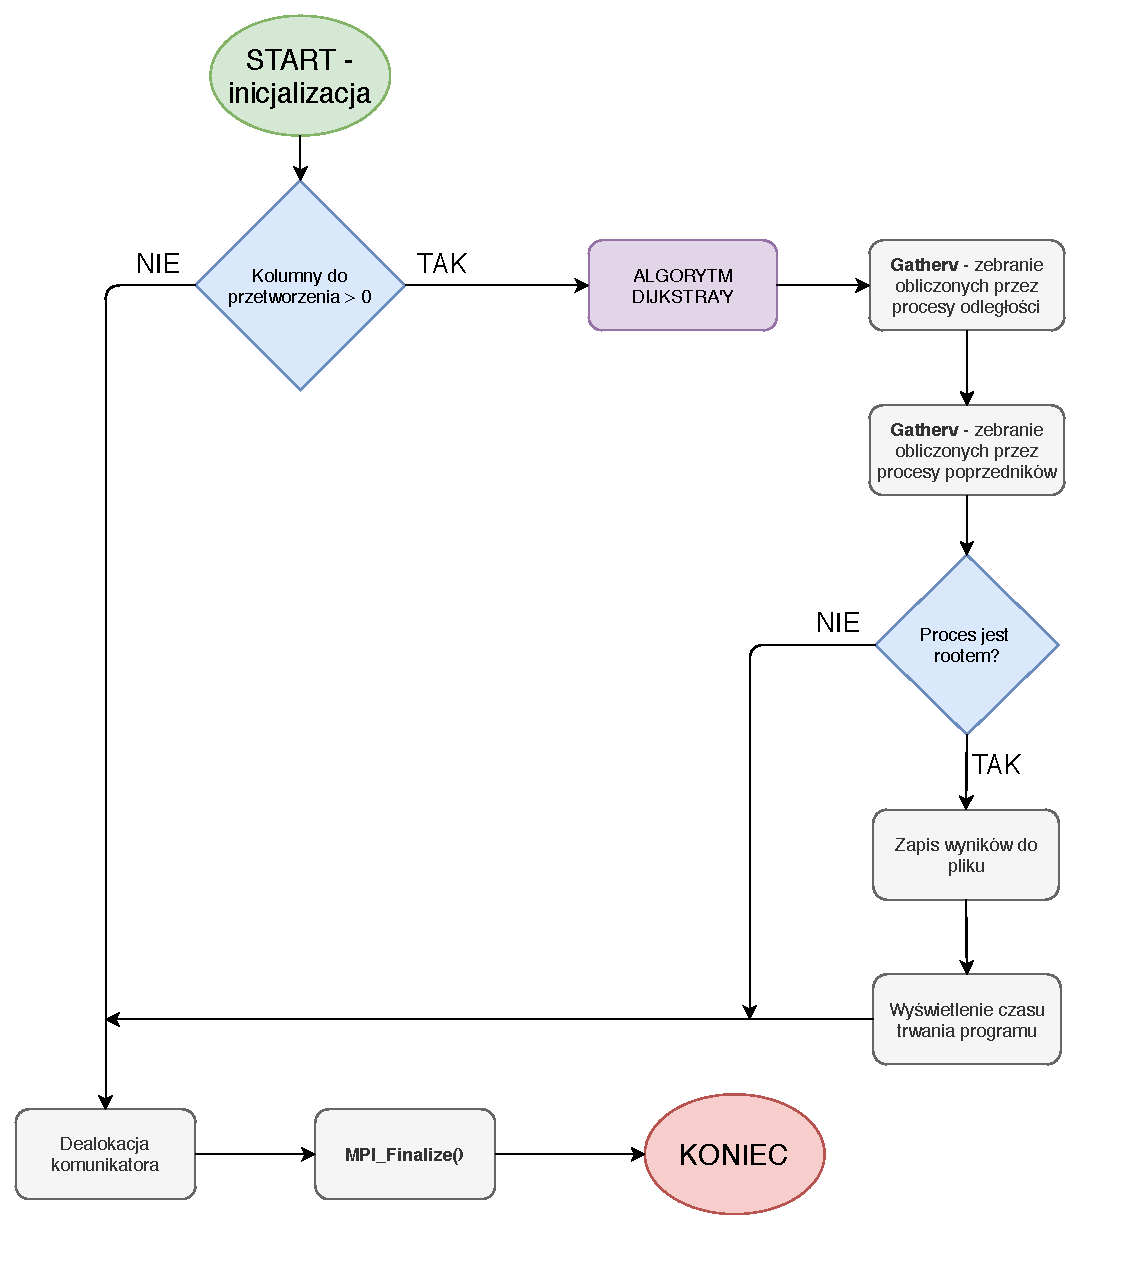
\includegraphics[width=\textwidth]{static/Diagram2.pdf}
\caption{Schemat blokowy ilustrujący przebieg głównej części programu wraz z zapisaniem wyników i zakończeniem. Schemat nie zawiera implementacji algorytmu Dijkstry.}
\label{fig:diagram2}
\end{figure}

\begin{figure}[H]
\centering
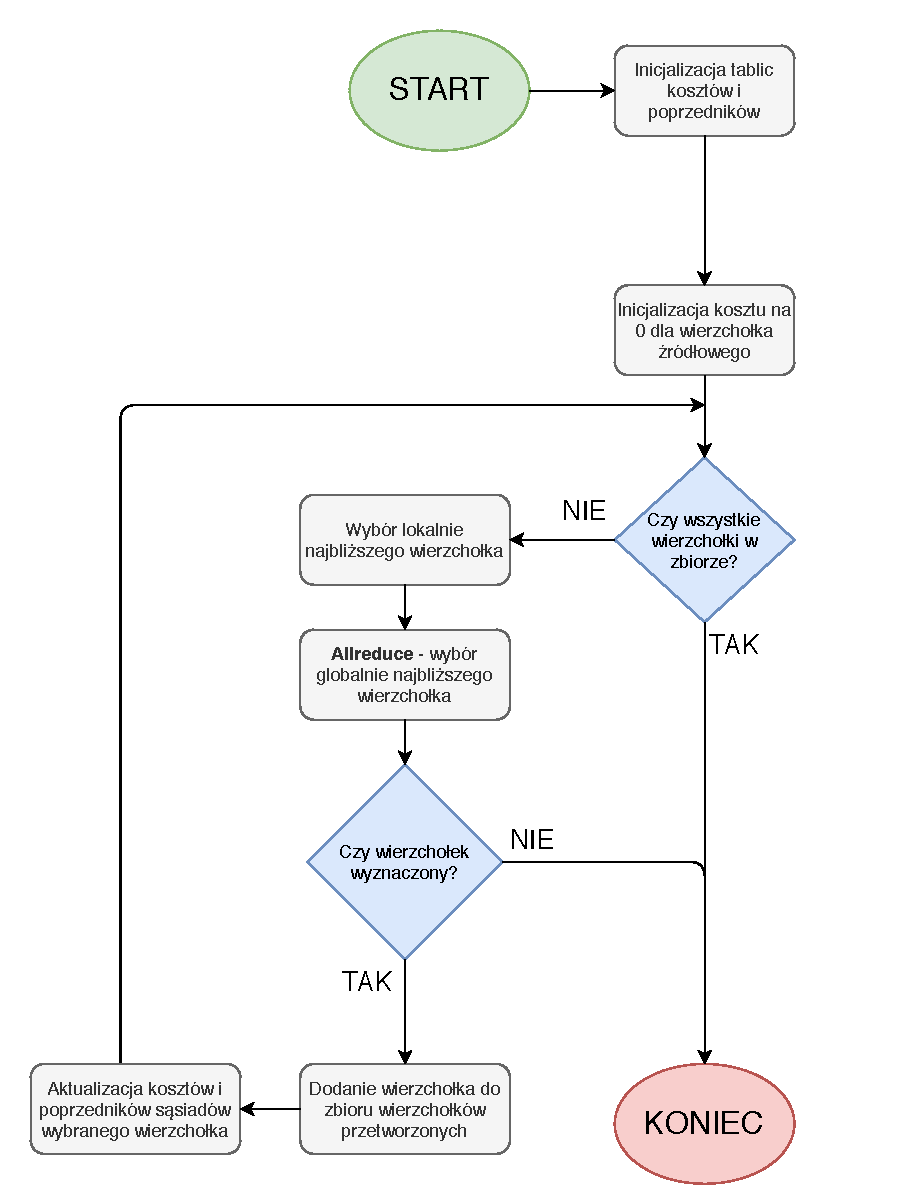
\includegraphics[width=0.9\textwidth]{static/Diagram3.pdf}
\caption{Schemat blokowy ilustrujący przebieg głównej pętli algorytmu Dijkstry.}
\label{fig:diagram3}
\end{figure}


\subsection{Zastosowane funkcjonalności MPI}
W ramach projektu zastosowane zostały następujące funkcjonalności MPI:
\begin{itemize}
\item operacja \lstinline{MPI_Bcast} - w celu rozesłania wszystkim procesom informacji o całkowitej ilości wierzchołków w przetwarzanym grafie
\item operacja \lstinline{MPI_Scatter} - w celu wysłania każdemu z procesów liczby przypisanych mu do obsłużenia wierzchołków grafu
\item operacja \lstinline{MPI_Scatterv} - celu wysłania każdemu z procesów danych z macierzy sąsiedztwa. Wymagana jest w tym przypadku możliwość wysłania każdemu z procesów danych o różnej długości.
\item operacja \lstinline{MPI_Allreduce} - w celu wyznaczenia wierzchołka o najmniejszej wartości kosztu
\item operacja \lstinline{MPI_Gatherv} - w celu zebrania wyników wyprodukowanych przez każdy z procesów. W tym przypadku wymagana jest możliwość odbioru od każdego z procesów danych i innej długości
\item operacje \lstinline{MPI_Comm_split} oraz \lstinline{MPI_Comm_free} - w celu utworzenia i zwolnienia nowego komunikatora. Pozwala to wykluczyć bierne (nadmiarowe) procesy z udziału w wykonywaniu algorytmu.
\end{itemize}

\section{Testy projektu}
\textbf{TODO:Wtorek}

\newpage
\section{Obsługa programu}
Niniejsza część dokumentacji przedstawia informacje związane z kompilacją i uruchomieniem projektu.

\subsection{Kompilacja}
Do kompilacji projektu został przygotowany plik \lstinline|CMakeLists.txt|. Za jego pomocą możliwe jest wygenerowanie pliku \lstinline{Makefile} służącego do kompilacji. Preferowanym sposobem użycia tego pliku jest tzw. użycie \textit{out-of-source} z katalogu \lstinline{build}. Znajdując się w katalogu głównym projektu należy wykonać następujące operacje:
\begin{lstlisting}
$ mkdir build
$ cd build
$ cmake ..
$ make
\end{lstlisting}

Aby kompilacja zakończyła się powodzeniem wymagane jest posiadanie zainstalowanej biblioteki \lstinline|MPI|. Na pracowni WFiIS konieczne jest ponadto załadowanie odpowiednich zmiennych środowiskowych przed kompilacją za pomocą polecenia:
\begin{lstlisting}
$ source /opt/nfs/config/source_mpich32.sh
\end{lstlisting}

W dalszej części przydatny może się również okazać plik zawierający informację o dostępnych węzłach. Na pracowni generuje się go za pomocą poniższej komendy:
\begin{lstlisting}
$ /opt/nfs/config/station_name_list.sh 201 216 > nodes
\end{lstlisting}

\subsection{Uruchomienie} \label{sec:uru}

Aby uruchomić program użytkownik może skorzystać z opcji udostępnianych przez wygenerowany plik \lstinline|Makefile|:
\begin{itemize}
\item  \lstinline|make runMPI| - uruchomiona zostaje równoległa wersja programu,
\item  \lstinline|make runSerial| - uruchomiona zostaje sekwencyjna wersja programu.
\end{itemize}

\noindent
Można skorzystać z domyślnych parametrów uruchomienia, lub podać własne:
\begin{itemize}
\item  \lstinline|VERTEX=V| - jako wierzchołek startowy zostanie wybrany wierzchołek \lstinline|V|, domyślną wartością jest $0$,
\item  \lstinline|FILE=F| - jako plik wejściowy zostanie użyty plik \lstinline|F|, plik domyślny to \lstinline{../data/graph.dat}
\item  \lstinline|N=N| - parametr \lstinline|mpiexec| ustalający ilość procesów, wartość domyślna jest równa $1$,
\item  \lstinline|HOSTS=H| -  parametr \lstinline|mpiexec|, plik wejściowy z węzłami.
\end{itemize}

\noindent
Przykładowe uruchomienie programu może wyglądać następująco:
\begin{lstlisting}
$ make runMPI VERTEX=1 FILE="../data/graph.dat" N=5
\end{lstlisting}

Jeśli użytkownik nie chce skorzystać z udostępnionych opcji można również uruchomić pliki wykonywalne samodzielnie. Po wykonaniu komendy \lstinline|make install-all| zostaną one udostępnione w katalogu z którego prowadzona była kompilacja. Jako argument należy podać kolejno numer wierzchołka startowego oraz plik wsadowy. Pierwszy argument jest obligatoryjny. Może to wyglądać np. tak jak poniżej:

\begin{lstlisting}
$ make install-all
$ mpiexec -n 5 ./DijkstraMPI 1 "../data/graph.dat"
\end{lstlisting}

Po uruchomieniu programu, jeśli zostało włączone logowanie, zostaną wyświetlone informacje na temat czasu wykonania. Znalezione ścieżki są zapisywane do plików: odpowiednio \lstinline|resultMPI.txt| oraz \lstinline|resultSerial.txt|.

\subsection{Dodatkowe opcje}
Korzystając z udostępnionego \lstinline|CMakeLists.txt| można również włączyć dodatkowe opcje, takie jak:
\begin{itemize}
\item \lstinline+-DBUILD_DOC=ON|OFF+ generowanie dokumentacji \lstinline|Doxygen|, domyślnie ta opcja jest wyłączona,
\item \lstinline+-DSHOULD_LOG=TRUE|FALSE+ włączenie/wyłączenie generowania logów.
\end{itemize}

\noindent
Dostępne są również dodatkowe opcje programu \lstinline|make|, takie jak:
\begin{itemize}
\item \lstinline| make clean-all | - przywrócenie zawartości podkatalogu do stanu wyjściowego,
\item \lstinline| make install-all | - udostępnienie plików wykonywalnych w podkatalogu,
\item \lstinline| make doc |  - wygenerowanie dokumentacji \lstinline|Doxygen|,
\item \lstinline| make runMPI |  - uruchomienie programu w wersji równoległej, opisane w punkcie \ref{sec:uru},
\item \lstinline| make runSerial |  - uruchomienie programu w wersji sekwencyjnej, opisane w punkcie  \ref{sec:uru},
\end{itemize}

\subsection{Dane wejściowe}
Program jako jedną z danych wejściowych przyjmuje plik z grafem zapisanym w postaci macierzy sąsiedztwa.
W pierwszej linii pliku powinna znajdować się ilość wierzchołków.

\begin{lstlisting}[caption={Przykładowy graf zapisany w odpowiednim formacie.}, captionpos=b ]
5
0.0000  0.0000  0.0000  8.2700  0.0000
4.2000  0.0000  8.5200  0.0000  0.0000
3.0700  0.0000  0.0000  0.0000  7.7700
0.0000  0.0000  7.4900  0.0000  0.0000
9.5700  6.9400  7.7900  6.6900  0.0000
\end{lstlisting}

Do wygenerowania pliku w takim formacie można użyć skryptu pomocniczego \lstinline|generateGraphs.py| opisanego w sekcji \ref{sec:gen_g}.

\subsection{Generowanie grafów} \label{sec:gen_g}
W ramach projektu został udostępniony dodatkowy skrypt  \lstinline|generateGraphs.py|. Służy on do generowania grafów skierowanych o wybranej przez użytkownika liczbie wierzchołków i krawędzi. Znajduje się on w katalogu \lstinline|\data|. Dostępne są opcje:
\begin{itemize}
\item \lstinline|-h| - pomoc skryptu,
\item \lstinline|-e| - liczba krawędzi w grafie, jeśli wartość nie została podana, ustawiana jest wartość domyślna $=10$,
\item \lstinline|-v| - liczba wierzchołków w grafie, wartość domyślna $=10$,
\item \lstinline|-f| - nazwa pliku wyjściowego, domyślna nazwa to \lstinline{graph.dat}.
\end{itemize}

Jeśli wartość krawędzi jest zbyt duża dla danej liczby wierzchołków, użytkownik zostaje poinformowany i zostaje ustawiona nowa, losowa wartość. Wagi krawędzi są nieujemnymi liczbami rzeczywistymi, z zakresu $[0, 10]$.

\begin{lstlisting}[caption={Pomoc skryptu \lstinline|generateGraphs.py|.}, captionpos=b ]
generateGraphs.py [-h] [-e E] [-v V] [-f FILE]

optional arguments:
	-h, --help            show this help message and exit
	-e E, --edges E       number of edges
	-v V, --vertices V    number of vertices
	-f FILE, --file FILE  name of output file
\end{lstlisting}

Grafy wygenerowane przy pomocy tego skryptu mogą zostać użyte jako dane wejściowe do programu.

\subsection{Obsługa programu na pracowni}
Z racji niedostępności programu \lstinline|CMake| na pracowni, zostały przygotowane dedykowane pliki \lstinline|Makefile| do obsługi programu. Plik przeznaczony do użycia przez użytkownika znajduje się w katalogu \lstinline|build_uni| wraz z odpowiednim plikiem do generacji dokumentacji.

\subsubsection{Skrypt Makefile}

Udostępnione zostały następujące opcje dla skryptu \lstinline|Makefile|:
\begin{itemize}
\item \lstinline|make install| - udostępnienie plików wykonywalnych w podkatalogu,
\item \lstinline|make runMPI|  -  uruchomienie programu w wersji równoległej, opisane w punkcie \ref{sec:uru},
\item \lstinline|make runSerial|  - uruchomienie programu w wersji sekwencyjnej, opisane w punkcie  \ref{sec:uru},
\item \lstinline|make docs| - wygenerowanie dokumentacji \lstinline|Doxygen|, 
\item \lstinline|make clean| - przywrócenie zawartości podkatalogu do stanu wyjściowego.
\end{itemize}

\subsubsection{Uruchomienie}
Aby uruchomić program z przykładowymi argumentami należy wykonać następujące operacje (zakładając, że użytkownik znajduje się w katalogu głównym projektu):
\begin{lstlisting}
$ cd build_uni
$ source /opt/nfs/config/source_mpich32.sh
$ make runMPI
\end{lstlisting}

Szczególnie istotnym punktem jest załadowanie odpowiednich zmiennych środowiskowych.

Uruchomienie programu bez użycia \lstinline|make runMPI| wygląda następująco:
\begin{lstlisting}
$ cd build_uni
$ source /opt/nfs/config/source_mpich32.sh
$ make installMPI
$ mpiexec -n 5 DijkstraMPI 1 "../data/graph.dat"
\end{lstlisting}

W podobny sposób jak powyższe możemy uruchomić wersję sekwencyjną, oczywiście z odpowiednim kompilatorem.

\subsubsection{Plik wejściowy z węzłami}

Aby wygenerować plik wejściowy z węzłami, który może zostać użyty do uruchomienia wersji równoległej należy wykonać następujące polecenia:
\begin{lstlisting}
$ cd build_uni
$ /opt/nfs/config/station_name_list.sh 201 216 > nodes
\end{lstlisting}

Tak wygenerowany plik można podać jako argument wykonania:
\begin{lstlisting}
$ make runMPI HOSTS="nodes"
\end{lstlisting}

\newpage
\begin{thebibliography}{9}
\bibitem{gramagupta} 
Ananth Grama, Anshul Gupta, George Karypis, Vipin Kumar 
\textit{Introduction to Parallel Computing, Second Edition}. 
Addison-Wesley, 2003.

\bibitem{millerpore} 
Aditya Pore, Russ Miller
\textit{Parallel implementation of Dijkstra's algorithm using MPI library on a cluster}.
Link: \url{https://cse.buffalo.edu/faculty/miller/Courses/CSE633/Pore-Spring-2014-CSE633.pdf} (dostęp: 21.04.2020)

\bibitem{zilongye}
Zilong Ye
\textit{An Implementation of Parallelizing Dijkstra’s Algorithm}.
Link: \url{https://cse.buffalo.edu/faculty/miller/Courses/CSE633/Ye-Fall-2012-CSE633.pdf} (dostęp: 21.04.2020)

\bibitem{wikipedia}
Wikipedia, The Free Encyclopedia
\textit{Dijkstra's algorithm}
Link: \url{https://en.wikipedia.org/wiki/Dijkstra\%27s_algorithm} (dostęp: 21.04.2020)

\bibitem{mpich}
Dokumentacja MPICH: \url{https://www.mpich.org/documentation/guides/} (dostęp: 21.04.2020)

\bibitem{msmpi}
Dokumentacja Microsoft MPI: \url{https://docs.microsoft.com/en-us/message-passing-interface/microsoft-mpi} (dostęp: 21.04.2020)

\bibitem{mpitutorial}
Wes Kendall
\textit{MPI Tutorial: MPI Scatter, Gather, and Allgather}.
Link: \url{https://mpitutorial.com/tutorials/mpi-scatter-gather-and-allgather/} (dostęp: 21.04.2020)

\bibitem{cppreference}
Dokumentacja języka C++ dostępna na stronie \url{https://en.cppreference.com/w/} (dostęp: 21.04.2020)


\end{thebibliography}

\end{document}